\section*{Introduction}

\addtocounter{chapter}{1}
\setcounter{figure}{0}

When one takes a historical perspective on language, one can observe
periods in time when the dominating language strategy for one subarea
of meaning is replaced by another strategy. This happened for example
in the history of the basic colour terms which simultaneously shifted
from a strategy that focussed on brightness to another strategy in
which the hue dimensions also became relevant. In order to model such
shifts, I explore the hypothesis in which agents track the
communicative success both at the level of linguistic items and the
level of the language strategies \citep{bleys09linguistic}.

\begin{figure}[htbp]
  \begin{center}
    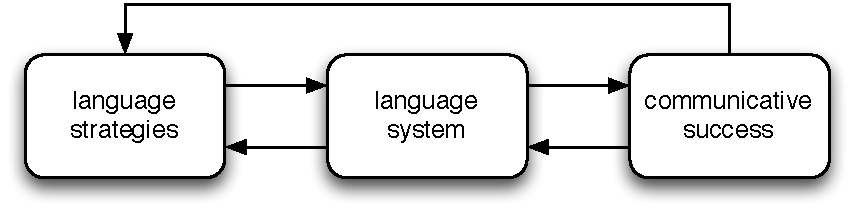
\includegraphics[width=0.65\textwidth]{./intro/figures/strategies-2.pdf}
    \caption[Several strategies competing to express the same subarea
    of meaning]{Several language strategies can compete to express the
      same subarea of meaning. This competition can be orchestrated
      through tracking the communicative success both at the level of
      the linguistic items in a language system and at the level of
      language strategies.}
    \label{f:strategies-2}
  \end{center}
\end{figure}

The next question is how new language strategies may come into
existence. The main theory that I will explore is the recruitment
theory \citep{steels07recruitment}, which states that general
cognitive operations can be recruited to solve linguistic
problems. This can be achieved through a combinatorial search process
of basic cognitive operations. This process is illustrated in Figure
\ref{f:strategies-3}.

\begin{figure}[htbp]
  \begin{center}
    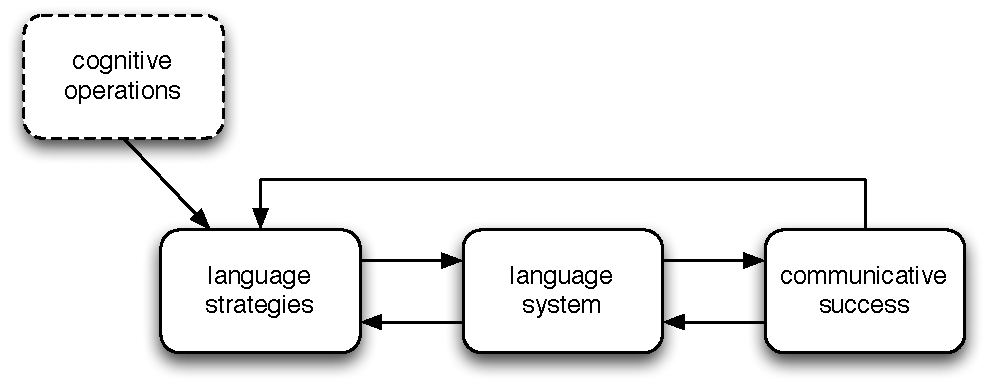
\includegraphics[width=0.65\textwidth]{./intro/figures/strategies-3.pdf}
    \caption[The origins of language strategies]{A language strategy
      can be generated through a combinatorial search process of
      cognitive operators}
    \label{f:strategies-3}
  \end{center}
\end{figure}

\addtocounter{chapter}{-1}

\thispagestyle{empty}